\section{Software framework}

\subsection{Implemented framework}
\begin{frame}{The implemented framework}{}
A software framework has been implemented (5k lines C++):
\begin{itemize}
  \item Receive UDP packets from electronics
  \item Consistency checks
  \item Event building(s)
  \item Execution of trigger algorithms (L1 and L2)
  \item Sending data to storage
\end{itemize}
\end{frame}

\subsection{Socket programming}
\begin{frame}{pf\_ring - new type of network socket}{}
	\begin{alertblock}{Bad performance with standard Kernel sockets}
		Interrupt based	transmission causes packet loss ($\approx 10^{-5}$)
	\end{alertblock}
	
	\begin{block}{Special socket: pf\_ring DNA by ntop}
		\begin{itemize}
		  \item Direct access to the NIC memory (avoids system calls)
		  \pro Only $\approx$40\% CPU @ full speed 10G receiving 1kB packets
		  \pro No packet loss at all
		  \contra Need to implement Ethernet, IP, UDP, ARP\ldots
		\end{itemize}
	\end{block}
	\begin{ergo}
		270kHz Eventbuilding rate with only about 3 cores \\
		$\Rightarrow$ much processing power left for L1 and L2	trigger
	\end{ergo}
\end{frame}


%\subsection{Parallel programming}
%\begin{frame}{Same problem with Mutex/Semaphore}{}
%	\begin{block}{Bad performance with Mutexes/Semaphores}
%		\begin{ergo}
%			Implemented lockless queues based on consumer-producer communications
%		\end{ergo}
%	\end{block}
%	\begin{center} 
%		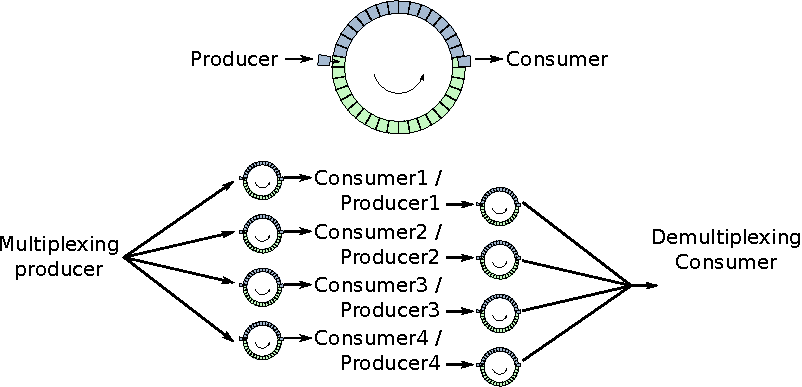
\includegraphics[height=4.5cm]{consumer-producer-queue}	
%	\end{center}
%\end{frame}
